\documentclass[12pt]{article}
% Modelo LaTeX para a matéria ENGF93.
% Desenvolvido por Silas Henrique (silash35@gmail.com),
% com contribuições de Daniel Diniz Santana (daniel.diniz@ufba.br).
% Versão 2026.06.28

\usepackage[brazilian]{babel}
\usepackage[T1]{fontenc}
\usepackage{graphicx}
\usepackage{csquotes}
\usepackage{amssymb,amsfonts,amsmath}
\usepackage{float}
\usepackage{booktabs}
\usepackage{indentfirst}

\usepackage{pdflscape}

\usepackage[titletoc,title]{appendix}
\renewcommand{\appendixname}{Apêndice}
\renewcommand{\appendixpagename}{Apêndices}
\renewcommand{\appendixtocname}{Apêndices}

\usepackage{geometry}
\geometry{
  a4paper,
  left=3cm,
  right=2cm,
  top=3cm,
  bottom=2cm,
  footskip=0cm
}

\usepackage{fancyhdr}
\usepackage{tikz}
\pagestyle{fancy}
\fancyhf{}
\fancyfoot[R]{\thepage}
\renewcommand{\headrulewidth}{0pt}

\fancypagestyle{paisagem}{
  \fancyhf{}
  \renewcommand{\headrulewidth}{0pt}
  \renewcommand{\footrulewidth}{0pt}
  \fancyfoot[C]{%
    \tikz[remember picture,overlay]
    \node[rotate=90] at ([xshift=-2cm, yshift=-2cm]current page.north east) {\thepage};
  }
}

\usepackage[backend=biber,style=abnt]{biblatex}
\addbibresource{../common/referencias.bib}
\addbibresource{../common/referencias2.bib}

\newcommand{\ua}{$\uparrow$}
\newcommand{\da}{$\downarrow$}

\makeatletter
\renewcommand{\maketitle}{
  \begin{center}
    \textbf{UNIVERSIDADE FEDERAL DA BAHIA}\\
    \textbf{ESCOLA POLITÉCNICA}\\
    \textbf{ENGENHARIA DE CONTROLE E AUTOMAÇÃO DE PROCESSOS}\\
    \textbf{ENGF93 – ANÁLISE DE PROCESSOS E SISTEMAS I}

    \vspace{9cm}

    \textbf{\LARGE \@title}

    \vfill

    \begin{flushleft}
      \@author
    \end{flushleft}

    \vspace{2cm}

    Salvador, \@date
  \end{center}

  \thispagestyle{empty}
  \newpage
}
\makeatother


\title{Análise de um Sistema de Dois Reatores e um Separador com Reciclo}
\author{
  Silas Henrique Alves Araújo \\
  Guilherme Rocha Ribeiro
}
\date{\today}

\begin{document}

% CAPA
\maketitle

% SUMÁRIO
\tableofcontents
\thispagestyle{empty}
\newpage

% CONTEÚDO
\setcounter{page}{1}

\begin{abstract}
  Sistemas reator-separador com corrente de reciclo apresentam elevada relevância industrial, pois a recirculação de reagentes pode favorecer o aumento da conversão global e da seletividade do processo.
  Entretanto, o forte acoplamento entre reação, separação e reciclo torna sua dinâmica mais sensível às condições operacionais, exigindo uma análise cuidadosa de seu comportamento.
  Este trabalho caracteriza a dinâmica de um sistema composto por dois reatores contínuos de tanque agitado e um separador, integrados por uma corrente de reciclo, empregando ferramentas clássicas de análise de sistemas lineares nos domínios do tempo contínuo, da frequência e do tempo discreto.
  O modelo fenomenológico não linear foi simulado em malha aberta para identificar qualitativamente a influência de cada entrada sobre os estados do processo.
  Em seguida, a partir do modelo linearizado, obteve-se a matriz de funções de transferência, que permitiu verificar a estabilidade do sistema, determinar a solução analítica da resposta temporal e identificar suas principais características dinâmicas.
  No domínio da frequência, o diagrama de Bode permitiu analisar a resposta do sistema a diferentes frequências, enquanto a Transformada de Fourier fundamentou o desenvolvimento de filtros passa-baixa para atenuação de ruído.
  Já a discretização, com período de amostragem definido com base no teorema de Shannon, preservou as principais características transitórias da resposta contínua, enquanto o mapeamento dos polos para o plano z confirmou a estabilidade da representação discreta.
  Os resultados demonstram que as ferramentas de análise de sistemas lineares permitiram caracterizar a dinâmica do sistema reator-separador com reciclo nos domínios do tempo, da frequência e do tempo discreto.
  Conclui-se que essa caracterização amplia a compreensão do comportamento dinâmico do processo.

  \noindent
  \textbf{Palavras-chave}: reator-separador; reciclo; dinâmica de processos; estabilidade.
\end{abstract}

\section{Introdução}

% Parágrafo 1: Relevância industrial dos sistemas reator-separador com reciclo.

% Parágrafo 2: Problemática: o reciclo torna a dinâmica complexa e sensível à operação.

% Parágrafo 3: Desafios de controle: sistema MIMO acoplado, com respostas inversas e zeros no semiplano direito.

% Parágrafo 4: Ferramentas de anáise em espaço de estados e necessidade de observador para estados não medidos.

% Parágrafo 5: Objetivo do trabalho.

\section{Descrição do Sistema}

O sistema analisado é baseado em um processo químico composto por dois reatores contínuos de tanque agitado (CSTRs) conectados a um separador, conforme \textcite{pourkargar_2017} e a Figura~\ref{fig:diagram}.
Nele ocorrem duas reações exotérmicas consecutivas, $A \rightarrow B \rightarrow C$, em que $B$ é o produto de interesse e $C$ um subproduto.
Uma corrente de reciclo retorna do separador ao primeiro reator, e uma corrente de purga evita o acúmulo de subprodutos.

\begin{figure}[ht]
  \centering
  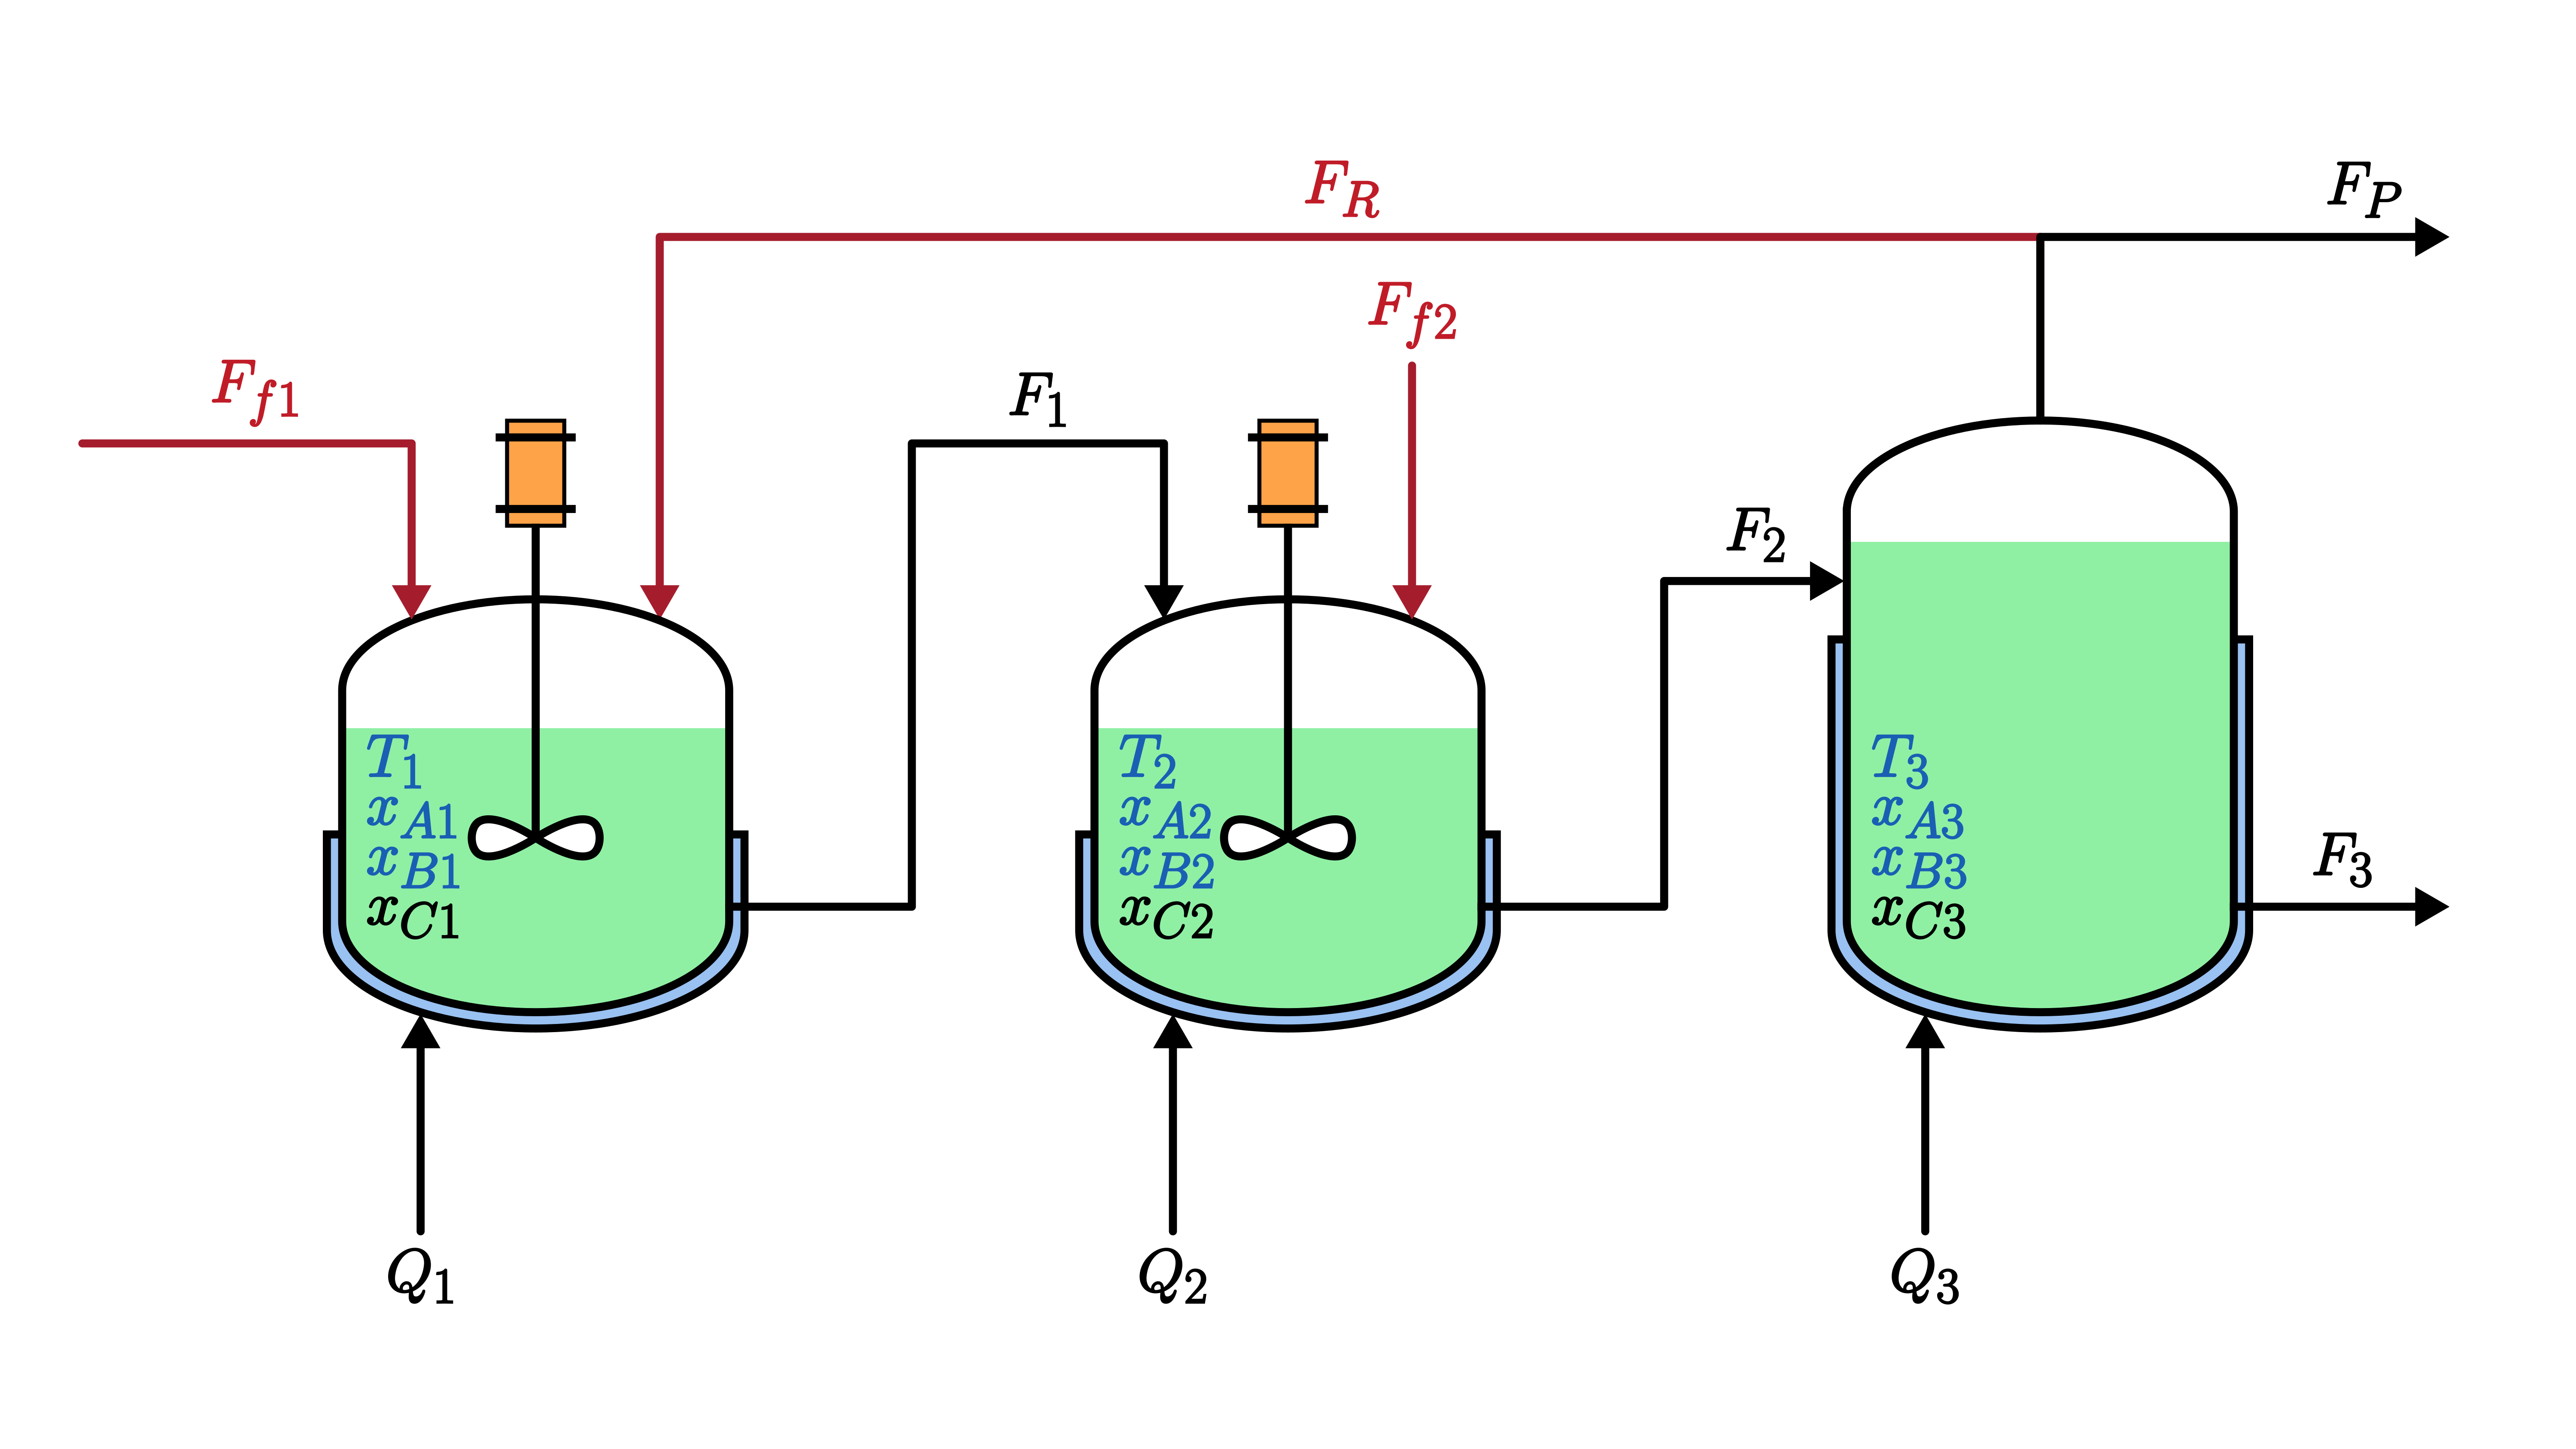
\includegraphics[width=0.6\textwidth]{../../figures/diagram.png}
  \caption{Diagrama do sistema integrado reator-separador utilizado neste trabalho.}
  \label{fig:diagram}
\end{figure}

As entradas do sistema são as vazões de alimentação $F_{f1}$ e $F_{f2}$ e a vazão de reciclo $F_R$, destacadas em vermelho na Figura~\ref{fig:diagram}.
As taxas de calor $Q_i$ e a temperatura de alimentação $T_0$ são mantidas constantes nos valores nominais.
As saídas são os estados de temperatura $T_i$ e de fração molar $x_{Ai}$ e $x_{Bi}$, em que $i = 1, 2, 3$ indica o primeiro reator, o segundo reator e o separador, respectivamente.

A dinâmica é descrita por equações diferenciais não lineares obtidas de balanços de massa e energia, com coeficientes de velocidade de reação dados pela lei de Arrhenius.
O modelo completo e os parâmetros, extraídos de \textcite{pourkargar_2017}, são apresentados no Apêndice~\ref{sec:apendice_modelo}.

Como os volumes $V_i$ têm comportamento integrador, assume-se volume constante, e as vazões internas passam a ser relações algébricas:
\begin{align}
  F_1 & = F_{f1} + F_R    \\
  F_2 & = F_{f2} + F_1    \\
  F_3 & = F_2 - F_P - F_R
\end{align}
com $F_P = \varepsilon F_R$.
Obtém-se assim um modelo MIMO com três entradas e nove estados, tomados como saídas.

\section{Análise no Tempo Contínuo}

\subsection{Representação em Espaço de Estados}

O modelo não linear foi linearizado por expansão em série de Taylor de primeira ordem em torno do ponto de operação em regime estacionário apresentado no Apêndice~\ref{sec:apendice_ponto_operacao}.
Em termos das variáveis de desvio, o modelo linearizado assume a forma de espaço de estados
\begin{align}
  \dot{\mathbf{x}}(t) & = \mathbf{A}\,\mathbf{x}(t) + \mathbf{B}\,\mathbf{u}(t), \\
  \mathbf{y}(t)       & = \mathbf{C}\,\mathbf{x}(t),
\end{align}
em que $\mathbf{x}(t) \in \mathbb{R}^{9}$ é o vetor de estados, $\mathbf{u}(t) \in \mathbb{R}^{3}$ é o vetor de entradas e $\mathbf{y}(t) \in \mathbb{R}^{9}$ é o vetor de saídas, todos em desvio em relação ao ponto de operação.
As matrizes $\mathbf{A} \in \mathbb{R}^{9 \times 9}$, $\mathbf{B} \in \mathbb{R}^{9 \times 3}$ e $\mathbf{C} \in \mathbb{R}^{9 \times 9}$ são, respectivamente, as matrizes de estado, de entrada e de saída.

As entradas do sistema são as vazões de alimentação e de reciclo,
\begin{equation}
  \mathbf{u} = \begin{bmatrix} F_{f1} & F_{f2} & F_R \end{bmatrix}^\top,
\end{equation}
e os estados são as temperaturas e as frações molares dos componentes $A$ e $B$ nas três unidades,
\begin{equation}
  \mathbf{x} = \begin{bmatrix} T_1 & T_2 & T_3 & x_{A1} & x_{B1} & x_{A2} & x_{B2} & x_{A3} & x_{B3} \end{bmatrix}^\top.
\end{equation}

Como todos os estados são tomados como saídas, tem-se $\mathbf{y} = \mathbf{x}$ e, portanto, $\mathbf{C} = \mathbf{I}_{9}$, a matriz identidade de ordem 9.
As matrizes $\mathbf{A}$, $\mathbf{B}$ e $\mathbf{C}$ completas são apresentadas no Apêndice~\ref{sec:apendice_ABC}.

A Figura~\ref{fig:lin_vs_nlin} compara as respostas dos modelos linear e não linear de $x_{B1}$ a degraus em $F_{f1}$.
Para a perturbação pequena, o modelo linearizado reproduz bem o comportamento não linear, o que confirma sua validade na vizinhança do ponto de operação.
À medida que a perturbação se afasta do ponto de operação, porém, os modelos divergem, e o modelo linear chega a prever uma fração molar negativa, sem significado físico.
Ao retornar ao valor nominal, as respostas voltam a coincidir.
Assim, o modelo linearizado é adequado apenas para pequenas variações em torno do ponto de operação.

\begin{figure}[ht]
  \centering
  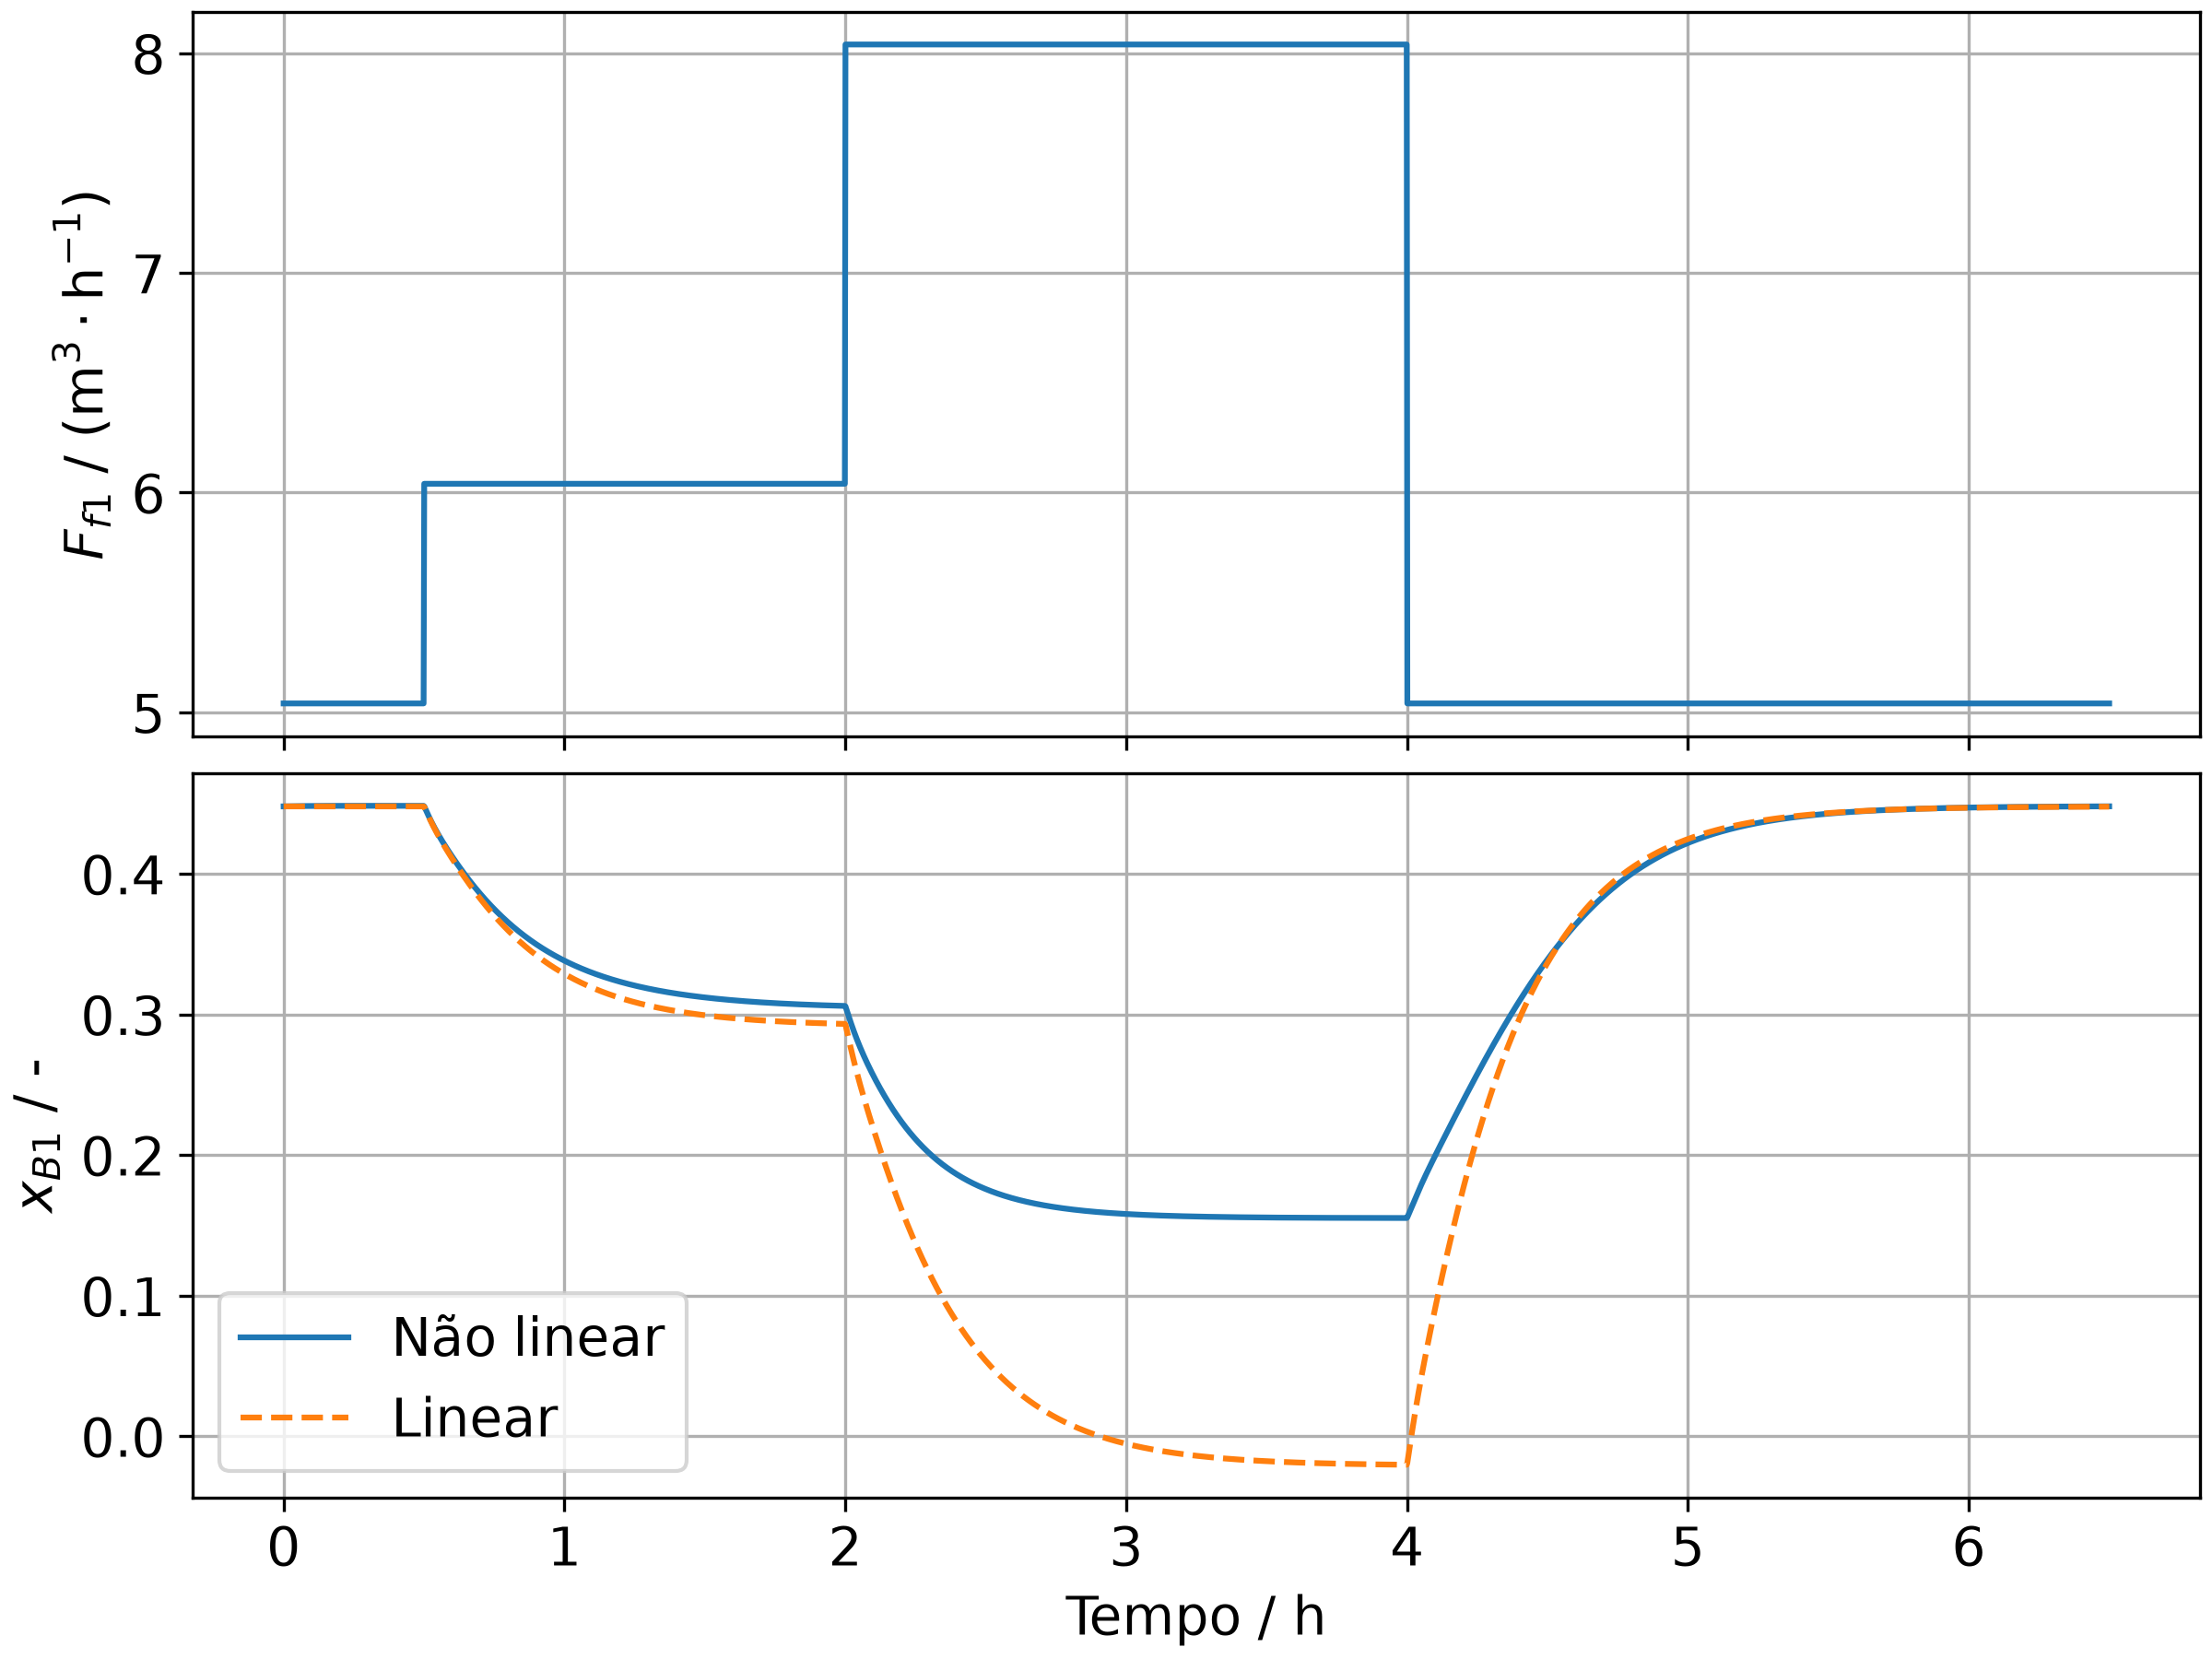
\includegraphics[width=0.6\textwidth]{../../figures/linear_vs_nonlinear/xB1_Ff1.png}
  \caption{Comparação entre as respostas dos modelos linear e não linear da fração molar $x_{B1}$ a degraus na vazão de alimentação $F_{f1}$: entrada (acima) e saída (abaixo).}
  \label{fig:lin_vs_nlin}
\end{figure}

\subsection{Estabilidade}

\subsection{Mapa de fase}

\section{Modelo Discreto}


\section{Controlabilidade}

\subsection{Análise de controlabilidade}

\subsection{Projeto do Controlador}

\section{Observabilidade}

\subsection{Análise de observabilidade}

\subsection{Projeto do observador}

\section{Conclusão}

% Parágrafo 1: Síntese do trabalho

% Parágrafo 2: Resumo dos principais resultados

% Parágrafo 3: Fechamento com objetivos atendidos e trabalhos futuros.

\section{Referências}
\printbibliography[heading=none]

\newpage

\appendix

\appendixpage
\addappheadtotoc

\section{Modelo fenomenológico do sistema reator-separador}
\label{sec:apendice_modelo}

O modelo fenomenológico completo da rede reator-separador, formulado por \textcite{pourkargar_2017}, é constituído por doze equações diferenciais, deduzidas a partir de balanços de massa e de energia nos reatores e no separador:
\begin{align}
  \frac{dV_1}{dt}    & = F_{f1} + F_R - F_1                                                                                                                                               \\
  \frac{dV_2}{dt}    & = F_{f2} + F_1 - F_2                                                                                                                                               \\
  \frac{dV_3}{dt}    & = F_2 - F_P - F_R - F_3                                                                                                                                            \\
  \frac{dT_1}{dt}    & = \frac{F_{f1}}{V_1}(T_0 - T_1) + \frac{F_R}{V_1}(T_3 - T_1) + \frac{Q_1}{\rho C_p V_1} - \frac{m}{C_p}(k_{11} x_{A1} \Delta H_{r1} + k_{21} x_{B1} \Delta H_{r2}) \\
  \frac{dT_2}{dt}    & = \frac{F_{f2}}{V_2}(T_0 - T_2) + \frac{F_1}{V_2}(T_1 - T_2) + \frac{Q_2}{\rho C_p V_2} - \frac{m}{C_p}(k_{12} x_{A2} \Delta H_{r1} + k_{22} x_{B2} \Delta H_{r2}) \\
  \frac{dT_3}{dt}    & = \frac{F_2}{V_3}(T_2 - T_3) + \frac{Q_3}{\rho C_p V_3}                                                                                                            \\
  \frac{dx_{A1}}{dt} & = \frac{F_{f1}}{V_1}(x_{A0} - x_{A1}) + \frac{F_R}{V_1}(x_{AR} - x_{A1}) - k_{11} x_{A1}                                                                           \\
  \frac{dx_{B1}}{dt} & = \frac{F_R}{V_1}(x_{BR} - x_{B1}) - \frac{F_{f1}}{V_1} x_{B1} + k_{11} x_{A1} - k_{21} x_{B1}                                                                     \\
  \frac{dx_{A2}}{dt} & = \frac{F_{f2}}{V_2}(x_{A0} - x_{A2}) + \frac{F_1}{V_2}(x_{A1} - x_{A2}) - k_{12} x_{A2}                                                                           \\
  \frac{dx_{B2}}{dt} & = \frac{F_1}{V_2}(x_{B1} - x_{B2}) - \frac{F_{f2}}{V_2} x_{B2} + k_{12} x_{A2} - k_{22} x_{B2}                                                                     \\
  \frac{dx_{A3}}{dt} & = \frac{F_2}{V_3}(x_{A2} - x_{A3}) - \frac{F_P + F_R}{V_3}(x_{AR} - x_{A3})                                                                                        \\
  \frac{dx_{B3}}{dt} & = \frac{F_2}{V_3}(x_{B2} - x_{B3}) - \frac{F_P + F_R}{V_3}(x_{BR} - x_{B3})
\end{align}
em que o índice $i$ identifica a unidade do processo: $i=1$ corresponde ao primeiro reator, $i=2$ ao segundo reator e $i=3$ ao separador.
Os termos $V_i$ e $T_i$ denotam, respectivamente, o volume e a temperatura de cada unidade, e $T_0$ é a temperatura da corrente de alimentação.
As vazões volumétricas de alimentação dos reatores são $F_{f1}$ e $F_{f2}$; $F_1$ e $F_2$ são as vazões que deixam os reatores 1 e 2, $F_3$ é a vazão de produto retirada do separador, $F_R$ é a vazão de reciclo e $F_P$, a de purga.
A taxa de calor fornecida a cada unidade é $Q_i$, ao passo que $\rho$ e $C_p$ são a massa específica e o calor específico do fluido, $m$ é a molalidade e $\Delta H_{rj}$ é a entalpia da reação $j$.
A composição do meio é dada pelas frações molares $x_{Ai}$ e $x_{Bi}$ dos componentes $A$ e $B$ na unidade $i$.
Por fim, $x_{A0}$ é a fração molar de $A$ na alimentação, $x_{AR}$ e $x_{BR}$ são as frações molares de $A$ e $B$ na corrente de reciclo e $k_{ri}$ é o coeficiente de velocidade da reação $r$ na unidade $i$.

Os coeficientes de velocidade das reações, $k_{ri}$, são funções da temperatura da unidade $i$ e seguem a lei de Arrhenius.
Os valores dos parâmetros são os reportados por \textcite{pourkargar_2017}.

\clearpage

\section{Ponto de Operação do Modelo}
\label{sec:apendice_ponto_operacao}

O ponto de operação em regime estacionário adotado para a linearização do sistema é o reportado por \textcite{pourkargar_2017}.
Os valores das entradas e dos estados nesse ponto constam, respectivamente, nas Tabelas~\ref{tab:u_ss} e \ref{tab:y_ss}.

\begin{table}[h]
  \caption{Valores das variáveis de entrada no ponto de operação em regime estacionário ($u_{ss}$).}
  \label{tab:u_ss}
  \centering
  \begin{tabular}{lll}
    \hline
    Variável & Valor   & Unidade \\
    \hline
    $F_{f1}$ & 5{,}04  & m³/h    \\
    $F_{f2}$ & 5{,}04  & m³/h    \\
    $F_R$    & 17{,}00 & m³/h    \\
    \hline
  \end{tabular}
\end{table}


\begin{table}[h]
  \caption{Valores dos estados do sistema no ponto de operação em regime estacionário ($y_{ss}$).}
  \label{tab:y_ss}
  \centering
  \begin{tabular}{lll}
    \hline
    Variável & Valor   & Unidade \\
    \hline
    $T_1$    & 432{,}4 & K       \\
    $T_2$    & 427{,}1 & K       \\
    $T_3$    & 432{,}1 & K       \\
    $x_{A1}$ & 0{,}536 & --      \\
    $x_{B1}$ & 0{,}448 & --      \\
    $x_{A2}$ & 0{,}545 & --      \\
    $x_{B2}$ & 0{,}438 & --      \\
    $x_{A3}$ & 0{,}298 & --      \\
    $x_{B3}$ & 0{,}670 & --      \\
    \hline
  \end{tabular}
\end{table}


\clearpage


\end{document}
